\Chapter{PREMIER PASSAGE EN DIFFUSION AVEC SAUTS}\label{sec:FPT_Jump}
Ce chapitre se concentre sur la variante discontinue du \acs{CIR}. Le processus est donc défini comme suit:
\begin{equation}\label{jump_cir_sde}
    X(t)=X(0)+\int_0^t a(b-X(s))ds+\int_0^t\sigma\sqrt{X(s)}dW(s)+J(t)
\end{equation}
avec
\begin{itemize}
    \item $X(0)=x$;
    \item $W(t)$ un \acs{MBS};
    \item $J(t)$ un processus de sauts pur:
    \[
    J(t)=\sum_{i=1}^{N(t)}Y_i
    \]
    où:
    \begin{itemize}
        \item $N(t)$ est un processus de poisson de paramètre $\lambda$;
        \item $Y_i$ des variables indépendantes et distribuées suivant une certaine loi.
    \end{itemize}
\end{itemize}

\section{Fonction Temps moyen \textemdash~Sauts uniformes descendants}\label{subsection_mean_jumps}
\subsection{Résolution du problème}
Dans cette section, la variante du \ac{CIR} avec sauts considérée est celle avec des sauts négatifs modélisés par des variables uniformément distribuées $Y_i\sim U[-x,0]$.

\paragraph{Dérivation de l'équation à résoudre}\phantom{}\\
En reprenant ce qui avait été fait en (\ref{section_fgm_eq}) pour dériver l'\acs{EDO} régissant la \acl{FGM} de $\tau(x)$, il est possible d'écrire:
\[
\frac{1}{2}\sigma^2 xM''(x;\alpha)+a(b-x)M'(x;\alpha)+\lambda\left\{\frac{1}{x}\int_{-x}^0M(x+y;\alpha)dy-M(x;\alpha)\right\}-\alpha M(x;\alpha)=0
\]
avec $M(0;\alpha)=M(c;\alpha)=1$.

Ensuite, en procédant comme dans (\ref{section_mean_eq}), il découle l'équation du temps moyen de sortie de l'intervalle pour le processus avec sauts:
\begin{equation}\label{mean_ide}
    \frac{1}{2}\sigma^2 xm''(x)+a(b-x)m'(x)+\lambda\left\{\frac{1}{x}\int_{-x}^0m(x+y)dy-m(x)\right\}=-1
\end{equation}
avec $m(0)=m(c)=0$.

Soit le changement de variable suivant:
\begin{equation}\label{variable_change_mean}
    \int_{-x}^0m(x+y)dy=\int_0^x m(z)dz
\end{equation}
La formule de Leibniz permet d'écrire:
\[
\frac{d}{dx}\left(\int_0^x m(z)dz\right)=m(x)
\]
Donc, en dérivant les deux côtés de l'équation (\ref{mean_ide}) et en éliminant le retour à la moyenne ($a=0$), il découle une \acs{EDO} d'ordre 3:
\begin{equation}\label{mean_3rd_order}
    \frac{1}{2}\sigma^2xm'''(x)+\sigma^2m''(x)-\lambda m'(x)=-\frac{1}{x}
\end{equation}

\paragraph{Résolution}\phantom{}\\
Soit les valeurs suivantes des paramètres: $\sigma=\sqrt{2}$, $\lambda=1$ et $c=1$. \textit{Maple} donne comme solution:
\begin{equation}\label{sol_mean_with_jumps}
    m(x)=C_1I_0(2\sqrt{x})+C_2K_0(2\sqrt{x})+2\ln(2\sqrt{x})+C_3
\end{equation}
avec $C_1$, $C_2$, $C_3$ des constantes à déterminer et $I_0(\cdot)$, $K_0(\cdot)$ les fonctions de Bessel modifiées de première et seconde espèce respectivement (voir annexe~\ref{special_functions}).

Les constantes $C_1$, $C_2$ et $C_3$ sont déterminées en imposant les conditions aux limites $m(0)=m(1)=0$ ainsi qu'une condition supplémentaire $m(0.5)=r$. Ensuite, la valeur de $r$ permettant de satisfaire l'équation originale (\ref{mean_ide}) est trouvée: $r\simeq0.3281$.

\paragraph{Étude du cas sans sauts}\phantom{}\\
Afin de comparer l'effet de la présence des sauts, il est intéressant de résoudre le même problème en retirant ces derniers. Soit $m_0(x)$ le temps moyen de sortie du processus sans sauts. En considérant les mêmes valeurs des paramètres, l'équation à résoudre devient:
\begin{equation}\label{mean_3rd_order_without_jumps}
    xm_0''(x)=-1
\end{equation}
La solution qui satisfait $m_0(0)=m_0(1)=0$ est:
\begin{equation}\label{sol_mean_with_0_jumps}
    m_0(x)=-x\ln(x)
\end{equation}

\subsection{Validation de l'expression obtenue}
Les fonctions \( m(x) \) (avec sauts) et \( m_0(x) \) (sans sauts), données respectivement par (\ref{sol_mean_with_jumps}) et (\ref{sol_mean_with_0_jumps}), sont tracées.
\paragraph{Visualisation}\phantom{}
\begin{figure}[htb]
    \centering
    \begin{subfigure}{0.45\linewidth}
        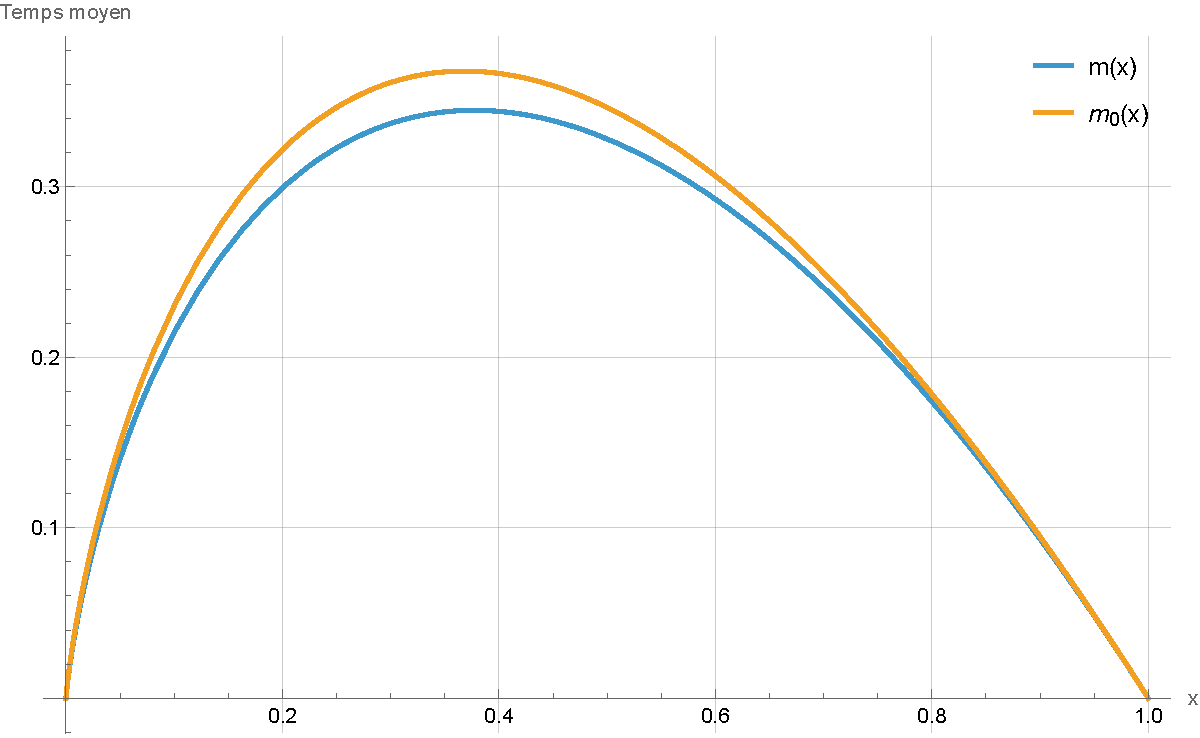
\includegraphics[width=\linewidth]{img/validation/Jumps/mean_jumps.pdf}
        \caption{Fréquence des sauts $\lambda=1$}
    \end{subfigure}
    \hfill
    \begin{subfigure}{0.45\linewidth}
        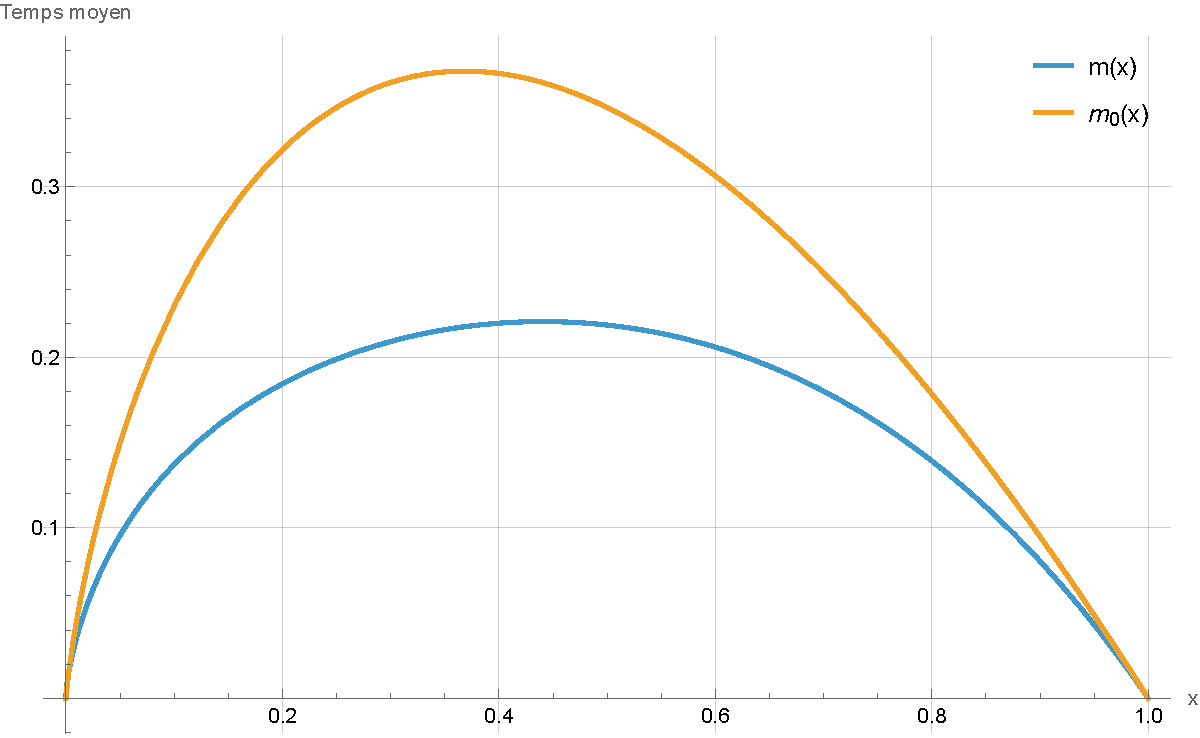
\includegraphics[width=\linewidth]{img/validation/Jumps/mean_big_jumps.pdf}
        \caption{Fréquence des sauts $\lambda=10$}
    \end{subfigure}
    \caption{Visualisation des temps moyens de sortie $m(x)$ et $m_0(x)$}\label{fig:JumpsMeanVisualisation}
\end{figure}
\FloatBarrier\paragraph{Analyse}\phantom{}\\
Il convient de souligner les observations suivantes:
\begin{itemize}
    \item Les conditions aux limites \( m(0) = m(c) = m_0(0) = m_0(c) = 0 \) sont bien vérifiées;
    \item Le temps moyen de sortie en présence de sauts ($m(x)$ en bleu) est inférieur à celui observé sans sauts ($m_0(x)$ en orange), ce qui illustre l'accélération du processus induite par ces derniers;
    \item Une augmentation de la fréquence des sauts $\lambda$ induit une diminution du temps moyen de sortie. Ce comportement est attendu comme les sauts augmente la probabilité que le \acs{CIR} quitte l'intervalle rapidement.
\end{itemize}
La fonction obtenue pour le temps moyen de sortie avec sauts est donc validée.

\section{Fonction Probabilité de sortie en zéro \textemdash~Sauts uniformes descendants}\label{subsection_probability_jumps}
\subsection{Résolution du problème}
Dans cette section, la variante du \ac{CIR} avec sauts considérée est identique à la précédente (sauts négatifs modélisés par des variables uniformément distribuées $Y_i\sim U[-x,0]$).

\paragraph{Dérivation de l'équation à résoudre}\phantom{}\\
Il est possible de montrer (voir~\cite{lefebvre2007}) que la fonction probabilité de sortie en zéro satisfait l'\acs{EDO}:
\begin{equation}\label{probability_ide}
    \frac{1}{2}\sigma^2xp''(x)+a(b-x)p'(x)+\lambda\left\{\frac{1}{x}\int_{-x}^0p(x+y)dy-p(x)\right\}=0
\end{equation}
sous les conditions $p(0)=1$ et $p(c)=0$.

Ensuite, en effectuant le même changement de variable que pour la fonction temps moyen (\ref{variable_change_mean}), en dérivant les deux membres de l'équation et en éliminant le retour à la moyenne ($a=0$), il découle:
\begin{equation}\label{probability_3rd_order}
    \frac{1}{2}\sigma^2xp'''(x)+\sigma^2p''(x)-\lambda p'(x)=0
\end{equation}
\paragraph{Résolution}\phantom{}\\
En reprenant les mêmes valeurs des paramètres ($\sigma=\sqrt{2}$, $\lambda=1$ et $c=1$) et en imposant les conditions $p(0)=1$, $p(1)=0$ et $p(0.5)=r$, \textit{Maple} donne la solution suivante:
\begin{equation}\label{sol_probability_with_jumps}
    p(x)=\frac{I_0(2)-I_0(2\sqrt{x})}{I_0(2)-1}
\end{equation}
avec $I_0(\cdot)$ la fonction de Bessel modifiée de première espèce (voir annexe~\ref{special_functions}) et $r\simeq0.5567$.
\paragraph{Étude du cas sans sauts}\phantom{}\\
Dans la même logique, le même problème en absence des sauts est résolu pour $p_0(x)=\mathds{P}[X(\tau(x))=0]$. L'équation (\ref{probability_3rd_order}) devient:
\[
xp_0''(x)=0
\]
La solution qui satisfait $p(0)=1$ et $p(1)=0$ est:
\begin{equation}\label{sol_probability}
    p_0(x)=1-x
\end{equation}
\subsection{Validation de l'expression obtenue}
Les fonctions \( p(x) \) (avec sauts) et \( p_0(x) \) (sans sauts), correspondant respectivement aux expressions (\ref{sol_probability_with_jumps}) et (\ref{sol_probability}), sont représentées graphiquement.
\paragraph{Visualisation}\phantom{}
\begin{figure}[htb]
    \centering
    \begin{subfigure}{0.45\linewidth}
        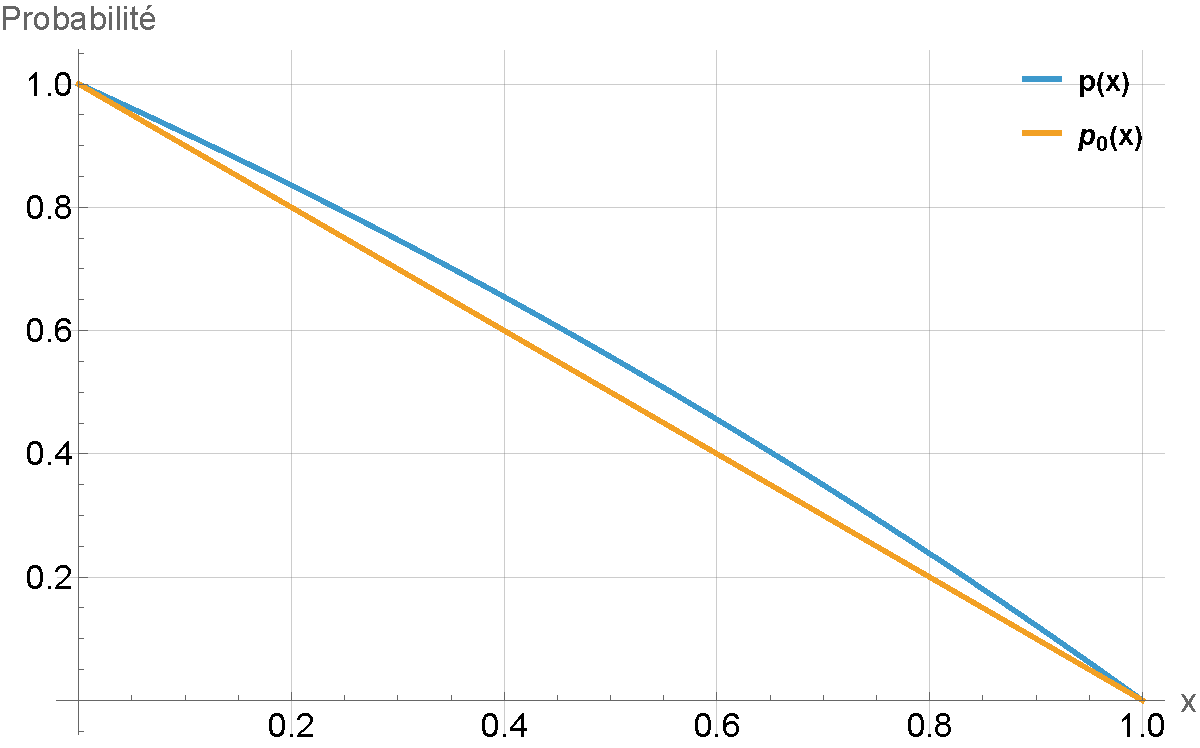
\includegraphics[width=\linewidth]{img/validation/Jumps/probability_jumps.pdf}
        \caption{Fréquence des sauts $\lambda=1$}
    \end{subfigure}
    \hfill
    \begin{subfigure}{0.45\linewidth}
        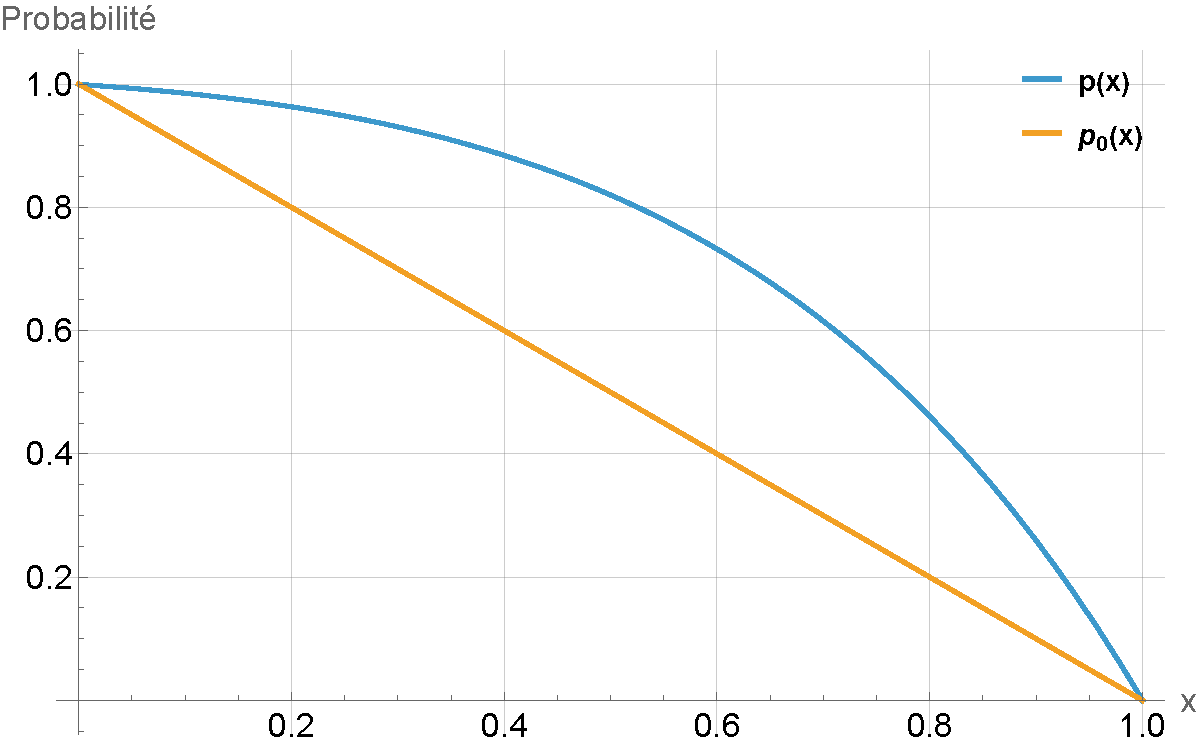
\includegraphics[width=\linewidth]{img/validation/Jumps/probability_big_jumps.pdf}
        \caption{Fréquence des sauts $\lambda=10$}
    \end{subfigure}
    \caption{Visualisation des probabilités de sortir en zéro $p(x)$ et $p_0(x)$}\label{fig:JumpsProbabilityVisualisation}
\end{figure}
\FloatBarrier\paragraph{Analyse}\mbox{}\\
Les observations suivantes peuvent être formulées:
\begin{itemize}
    \item Les conditions aux limites sont correctement satisfaites, à savoir \( p(0) = p_0(0) = 1 \) et \( p(c) = p_0(c) = 0 \);
    \item Les sauts étant négatifs, ils favorisent une sortie par la borne inférieure. La probabilité de franchissement par zéro est donc plus élevée dans le cas avec sauts ($p(x)$ en bleu);
    \item Une augmentation de la fréquence des sauts $\lambda$ entraîne une augmentation considérable de la probabilité de sortir par zéro. En effet, la multiplication des sauts tend à entraîner le processus vers la borne inférieure.
\end{itemize}
Ces résultats permettent donc de valider l'expression obtenue pour la probabilité de sortie en zéro.

\section{Fonction Dépassement Moyen \textemdash~Sauts exponentiels ascendants}
\subsection{Résolution du problème}
Dans cette section, la variante du \ac{CIR} avec sauts considérée est celle avec des sauts positifs modélisés par des variables aléatoires exponentielles $Y_i\sim \text{Exp}(\nu)$.

\paragraph{Dérivation de l'équation à résoudre}\phantom{}\\
Soit $f(x)=(x-c)_+$ la fonction mesurant un dépassement. En appliquant la formule de Dynkin (voir~\cite{dynkin1965}), il est possible d'écrire:
\begin{equation}\label{initial_dynkin}
    \mathds{E}[f(X(\tau(x)))]=f(x)+\mathds{E}\left[\int_0^{\tau(x)}\mathcal{L}f(X(s))ds\right]
\end{equation}
D'abord, en développant le terme de gauche, l'expression de la fonction $D(x)$ définie en (\ref{overshoot}) est retrouvée:
\begin{equation}\label{dynkin_left_simplification}
    \begin{aligned}
        \mathds{E}[f(X(\tau(x)))]&=\mathds{E}\left[(X(\tau(x))-c)_+\right]\\
        &=D(x)
    \end{aligned}
\end{equation}
Ensuite, le terme de droite peut être simplifié: 
\begin{equation}\label{dynkin_right_simplification_1}
    X(0)=x\in(0,c)\implies f(x)=0
\end{equation}
Par ailleurs, en développant le générateur infinitésimal (voir annexe~\ref{infinitesimal_generator}) appliqué à la fonction $f(x)$, il découle que:
\begin{equation}\label{dynkin_right_simplification_2}
    \begin{aligned}
        \mathcal{L}f(x)&=\frac{1}{2}\sigma^2xf''(x)+a(b-x)f'(x)+\lambda\int_0^{+\infty}\left[f(x+y)-f(x)\right]\nu e^{-\nu y}dy \\
        &=\lambda\int_{c-x}^{+\infty}(x+y-c)\nu e^{-\nu y}dy \\
        &=\frac{\lambda}{\nu e^{\nu c}}e^{\nu x}
    \end{aligned}
\end{equation}
En prenant en compte (\ref{dynkin_left_simplification},~\ref{dynkin_right_simplification_1},~\ref{dynkin_right_simplification_2}), l'équation (\ref{initial_dynkin}) devient:
\begin{equation}\label{simplified_dynkin}
    D(x)=\frac{\lambda}{\nu e^{\nu c}}\mathds{E}\left[\int_0^{\tau(x)}e^{\nu X(s)}ds\right]
\end{equation}
Soit la fonction $g(x)$ définie par:
\begin{equation}\label{g_defintion}
    g(x):=\mathds{E}\left[\int_0^{\tau(x)}e^{\nu X(s)}ds\right]
\end{equation}
Comme les coefficients de dérive et de diffusion du processus \acs{CIR} vérifient les conditions d'unicité trajectorielle (voir annexe~\ref{trajecotry_uniqueness}) et les sauts exponentiels ont des moments finis, le travail présenté dans~\cite{abundo2013} peut être utilisé pour établir l'\acs{EID} du second ordre associée:
\begin{equation}\label{initial_overshoot_ide}
    \frac{1}{2}\sigma^2xg''(x)+a(b-x)g'(x)+\lambda\int_0^{+\infty}\left[g(x+y)-g(x)\right]\nu e^{-\nu y}dy=-e^{\nu x}
\end{equation}
En séparant l'intégrale, il découle:
\begin{equation}\label{overshoot_ide}
        \frac{1}{2}\sigma^2xg''(x)+a(b-x)g'(x)+\lambda\int_0^{+\infty}g(x+y)\nu e^{-\nu y}dy-\lambda g(x)=-e^{\nu x}
\end{equation}
Le changement de variable $z=x+y$ permet d'écrire:
\[
\int_0^{+\infty}g(x+y)\nu e^{-\nu y}dy=\nu e^{\nu x}\int_x^{+\infty}g(z)e^{-\nu z}dz
\]
Soit:
\begin{equation}\label{phi_simplification}
    \Phi(x):=\int_x^{+\infty}g(z)e^{-\nu z}dz
\end{equation}
La formule de Leibniz donne:
\begin{equation}\label{phi_derivation}
        \Phi'(x)=-g(x)e^{-\nu x}\implies g(x)=-e^{\nu x}\Phi'(x)
\end{equation}
En injectant (\ref{phi_simplification},~\ref{phi_derivation}) dans (\ref{overshoot_ide}), l'équation devient:
\begin{equation}\label{Phi_equation}
    \begin{aligned}
        \frac{1}{2}\sigma^2x\Phi'''(x)+\Phi''(x)\left[\nu\sigma^2x+a(b-x)\right]\\+\Phi'(x)\left[\frac{1}{2}\sigma^2\nu^2x+a\nu(b-x)-\lambda\right]-\lambda\nu \Phi(x)=1
    \end{aligned}
\end{equation}
Le fonction recherchée $g(x)$ ne dépend que de $\Phi'(x)$. En posant $\phi(x)=\Phi'(x)$ et en dérivant l'équation (\ref{Phi_equation}), il découle l'\acs{EDO} homogène linéaire d'ordre 3:
\begin{equation}\label{phi_equation}
    \begin{aligned}
        x \phi'''(x)+\phi''(x) \left[\left(\frac{2(\nu\sigma^2-a)}{\sigma^2}\right)x+\left(\frac{2ab+\sigma^2}{\sigma^2}\right)\right]\\+\phi'(x) \left[\left(\frac{\sigma^2\nu^2-2a\nu}{\sigma^2}\right)x+\left(\frac{2(\nu\sigma^2-a-\lambda+ab\nu)}{\sigma^2}\right)\right]\\+\phi(x) \left[\frac{\nu^2  \sigma ^2-2\nu(a+\lambda )}{\sigma^2}\right]=0
    \end{aligned}
\end{equation}
Les conditions $g(0)=g(c)=0$ deviennent $\phi(0)=\phi(c)=0$. Enfin
\[
\begin{aligned}
    D(x) &= \frac{\lambda}{\nu e^{\nu c}}g(x)\\
    &=-\frac{\lambda}{\nu e^{\nu c}}e^{\nu x}\phi(x)
\end{aligned}
\]
Cependant, une expression explicite pour $\phi(x)$, si elle existe, est très difficile à obtenir. Cela rend donc la résolution du problème général assez compliqué. 

\paragraph{Résolution approximative pour $a=0$}\phantom{}\\
En remplaçant $g(x+y)$ dans (\ref{initial_overshoot_ide}) par un développement de Taylor, il est possible de réécrire l'intégrale comme suit:
\[
\begin{aligned}
    \lambda\int_0^{+\infty}\left[g(x+y)-g(x)\right]\nu e^{-\nu y}dy&=\lambda\int_0^{+\infty}\left[\sum_{n=0}^{+\infty}\frac{y^n}{n!}\frac{d^n}{dx^n}g(x)-g(x)\right]\nu e^{-\nu y}dy\\
    &=\lambda\int_0^{+\infty}\left[\sum_{n=1}^{+\infty}\frac{y^n}{n!}\frac{d^n}{dx^n}g(x)\right]\nu e^{-\nu y}dy
\end{aligned}
\]
Ensuite, en échangeant la série et l'intégrale, le $n$-ème moment de $Y_i$ apparaît, permettant ainsi de simplifier l'expression:
\[
\begin{aligned}
    \lambda\int_0^{+\infty}\left[\sum_{n=1}^{+\infty}\frac{y^n}{n!}\frac{d^n}{dx^n}g(x)\right]\nu e^{-\nu y}dy&=\lambda\sum_{n=0}^{+\infty}\left[\frac{1}{n!}\frac{d^n}{dx^n}g(x)\int_0^{+\infty}y^n\nu e^{-\nu y}dy\right]\\
    &=\lambda\sum_{n=0}^{+\infty}\frac{1}{n!}\frac{d^n}{dx^n}g(x)\mathds{E}\left[Y_i^n\right]\\
    &=\lambda\sum_{n=0}^{+\infty}\frac{1}{\nu^n}\frac{d^n}{dx^n}g(x)
\end{aligned}
\]
Par ailleurs, en supposant que les sauts sont petits ($\nu$ est grand), il est possible d'approximer la somme obtenue de la façon suivante:
\[
\sum_{n=0}^{+\infty}\frac{1}{\nu^n}\frac{d^n}{dx^n}g(x)\approx\frac{1}{\nu}g'(x)+\frac{1}{\nu^2}g''(x)
\]
L'équation (\ref{initial_overshoot_ide}) devient:
\begin{equation}\label{final_overshoot_ode}
    \left(\frac{1}{2}\sigma^2x+\frac{\lambda}{\nu^2}\right)g''(x)+\left[a(b-x)+\frac{\lambda}{\nu}\right]g'(x) =-e^{\nu x}
\end{equation}
Cette \acs{EDO} de second ordre est non homogène avec des coefficients polynomiaux et un terme exponentiel. La solution explicite, si elle existe, est difficile à obtenir. Dans la suite, un cas particulier du problème est considéré.

En éliminant le retour à la moyenne ($a=0$), l'\acs{EDO} (\ref{final_overshoot_ode}) devient:
\begin{equation}\label{particular_overshoot_ode}
    \left(\frac{1}{2}\sigma^2x+\frac{\lambda}{\nu^2}\right)g''(x)+\frac{\lambda}{\nu}g'(x) =-e^{\nu x}
\end{equation}
\textit{Wolfram Mathematica} donne:
\[
\begin{aligned}
    g(x)=\frac{1}{{\nu\sigma^2(2\lambda-\nu\sigma^2)}}\Bigg[\sigma^2\left(-C_1 \left(2 \lambda +\nu ^2 \sigma ^2 x\right)^{1-\frac{2 \lambda }{\nu  \sigma ^2}}+C_2 \nu  \left(2 \lambda -\nu  \sigma ^2\right)-2 \nu  e^{\nu  x}\right) \\-2 e^{-\frac{2 \lambda }{\nu  \sigma ^2}} \left(2 \lambda +\nu ^2 \sigma ^2 x\right) E_{1-\frac{2 \lambda }{\nu  \sigma ^2}}\left(-\frac{2 \lambda }{\nu  \sigma ^2}-x \nu \right)\Bigg]
\end{aligned}
\]
avec $E_n(x)$ la fonction intégrale exponentielle (voir annexe~\ref{special_functions}). \\
Alors, la forme finale de l'expression de la fonction Dépassement Moyen est obtenue:
\begin{equation}\label{sol_overshoot}
    \begin{aligned}
            D(x)=\frac{\lambda}{{\nu^2\sigma^2e^{\nu c}(2\lambda-\nu\sigma^2)}}\Bigg[\sigma^2\left(-C_1 \left(2 \lambda +\nu ^2 \sigma ^2 x\right)^{1-\frac{2 \lambda }{\nu  \sigma ^2}}+C_2 \nu  \left(2 \lambda -\nu  \sigma ^2\right)-2 \nu  e^{\nu  x}\right) \\-2 e^{-\frac{2 \lambda }{\nu  \sigma ^2}} \left(2 \lambda +\nu ^2 \sigma ^2 x\right) E_{1-\frac{2 \lambda }{\nu  \sigma ^2}}\left(-\frac{2 \lambda }{\nu  \sigma ^2}-x \nu \right)\Bigg]
    \end{aligned}
\end{equation}

\paragraph{Détermination des constantes}\phantom{}\\
Les conditions aux limites $g(0)=g(c)=0$ (et donc $D(0)=D(c)=0$) permettent de déterminer les deux constantes $C_1$ et $C_2$. Étant donné la longueur des expressions obtenues, celles-ci ne seront pas détaillées dans le présent document.

\subsection{Validation de l'expression obtenue}
\paragraph{Visualisation}\phantom{}\\
Toujours dans la même optique de validation, la fonction approximative obtenue pour $D(x)$ en (\ref{sol_overshoot}) est tracée pour différentes valeurs de la fréquence des sauts $\lambda\in\{2,3,6\}$ ainsi que le paramètre de longueur des sauts $\nu\in\{5,10,15\}$.
\begin{figure}[htb]
    \centering
    \begin{subfigure}{0.45\linewidth}
        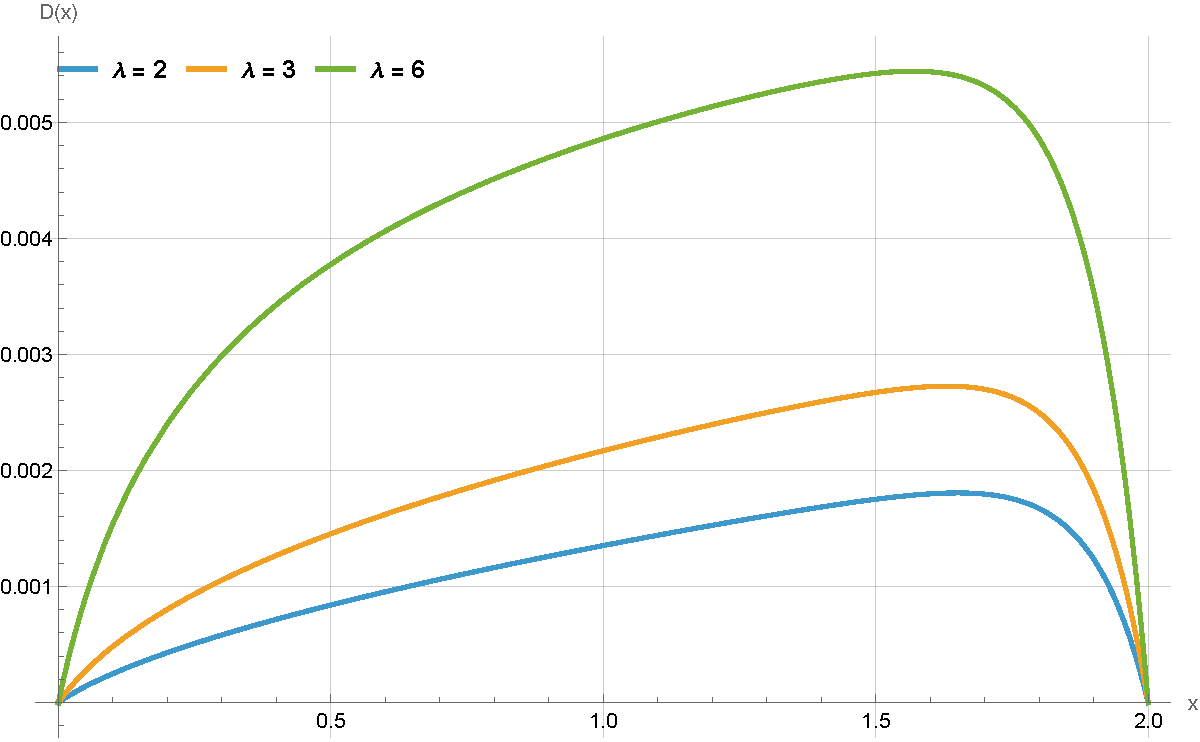
\includegraphics[width=\linewidth]{img/validation/Ovs/overshoot_lambda.pdf}
        \caption{Sensibilité de la fréquence des sauts $\lambda,\;\forall\;\lambda\in\{2,3,6\}$}\label{fig:Overshoot_lambda_visualisation}
    \end{subfigure}
    \hfill
    \begin{subfigure}{0.45\linewidth}
        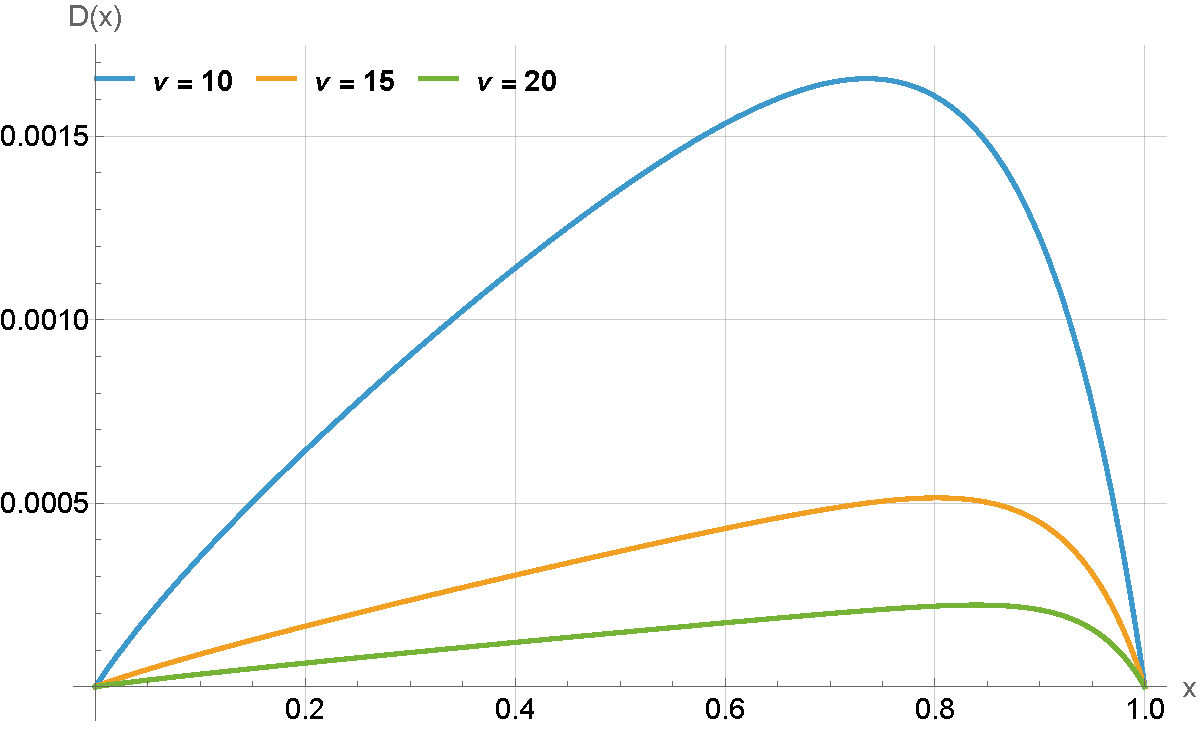
\includegraphics[width=\linewidth]{img/validation/Ovs/overshoot_nu.pdf}
        \caption{Sensibilité de la taille des sauts $\nu,\;\forall\;\nu\in\{5,10,15\}$}\label{fig:Overshoot_nu_visualisation}
    \end{subfigure}
    \hfill
    \caption{Visualisation de la fonction Dépassement Moyen $D(x)$}\label{fig:OvershootVisualisation}
\end{figure}
\FloatBarrier\paragraph{Analyse}\phantom{}\\
Les différents points suivants sont relevés:
\begin{itemize}
    \item Les conditions aux limites $D(0)=D(c)=0$ sont respectées;
    \item La fonction représente un \textit{dépassement moyen}, elle doit donc être positive pour toute valeur $x$ dans $[0,c]$;
    \item Une augmentation de la fréquence des sauts $\lambda$ induit une augmentation du dépassement moyen. En effet, il devient plus probable que le processus effectue un saut juste avant d'atteindre la frontière, ce qui augmente les chances de la franchir avec un certain excès;
    \item Une réduction de la taille des sauts (traduite par une augmentation de $\nu$) induit une diminution du dépassement moyen. En effet, même si un saut survient à proximité de la frontière, sa faible amplitude limite la distance franchie au-delà de celle-ci.
\end{itemize}
La fonction Dépassement Moyen $D(x)$ est donc validée.

